\documentclass[a4paper, 12pt]{article}
\usepackage[utf8]{inputenc}
\usepackage[english,russian]{babel}
\usepackage[warn]{mathtext}
\usepackage{graphicx}
\usepackage{float}
\usepackage{multirow}
\restylefloat{table}
\usepackage{amsmath}
\usepackage{floatflt}
\usepackage[T2A]{fontenc}
\usepackage[left=20mm, top=20mm, right=20mm, bottom=20mm, footskip=10mm]{geometry}

\tolerance 1414
\hbadness 1414
\emergencystretch 1.5em
\hfuzz 0.3pt        % размер максимального переполнения без warning'a
\widowpenalty=10000 % запрещает одиночную строку абзаца в начале страницы
\vfuzz \hfuzz
\raggedbottom       % если на странице мало содержимого, добавить пустое место в конце, а не в середине страницы



\begin{document}

\begin{titlepage}
	\centering
	\vspace{5cm}
	{\scshape\LARGE московский физико-технический институт (национальный исследовательский университет) \par}
	\vspace{6cm}
	{\scshape\Large Лабораторная работа 4.3.2 \par}
	{\huge\bfseries Дифракция света на ультразвуковых волнах \par}
	\vspace{1cm}
	\vfill
\begin{flushright}
	{\large Б03-102}\par
	\vspace{0.3cm}
	{\LARGE Куланов Александр}
\end{flushright}
	

	\vfill


	Долгопрудный, 2023 г.
\end{titlepage}

\begin{itemize}
	\item \textbf{Цель работы:} измерить координаты дифракционных полос, образующихся при дифракции света на акустической решетке, определить период этой решетки методом темного поля, рассчитать скорость ультразвука в воде
    \item \textbf{В работе используются:} оптическая скамья, осветитель, светофильтры, конденсор, щель, два длиннофокусных объектива, кювета с водой, кварцевый излучатель с микрометрическим винтом, генератор УЗ-частоты, частотомер, линза, отсчетное устройство, микроскоп.
\end{itemize}

\section{Экспериментальная установка}
\begin{figure}[H]
    \centering
    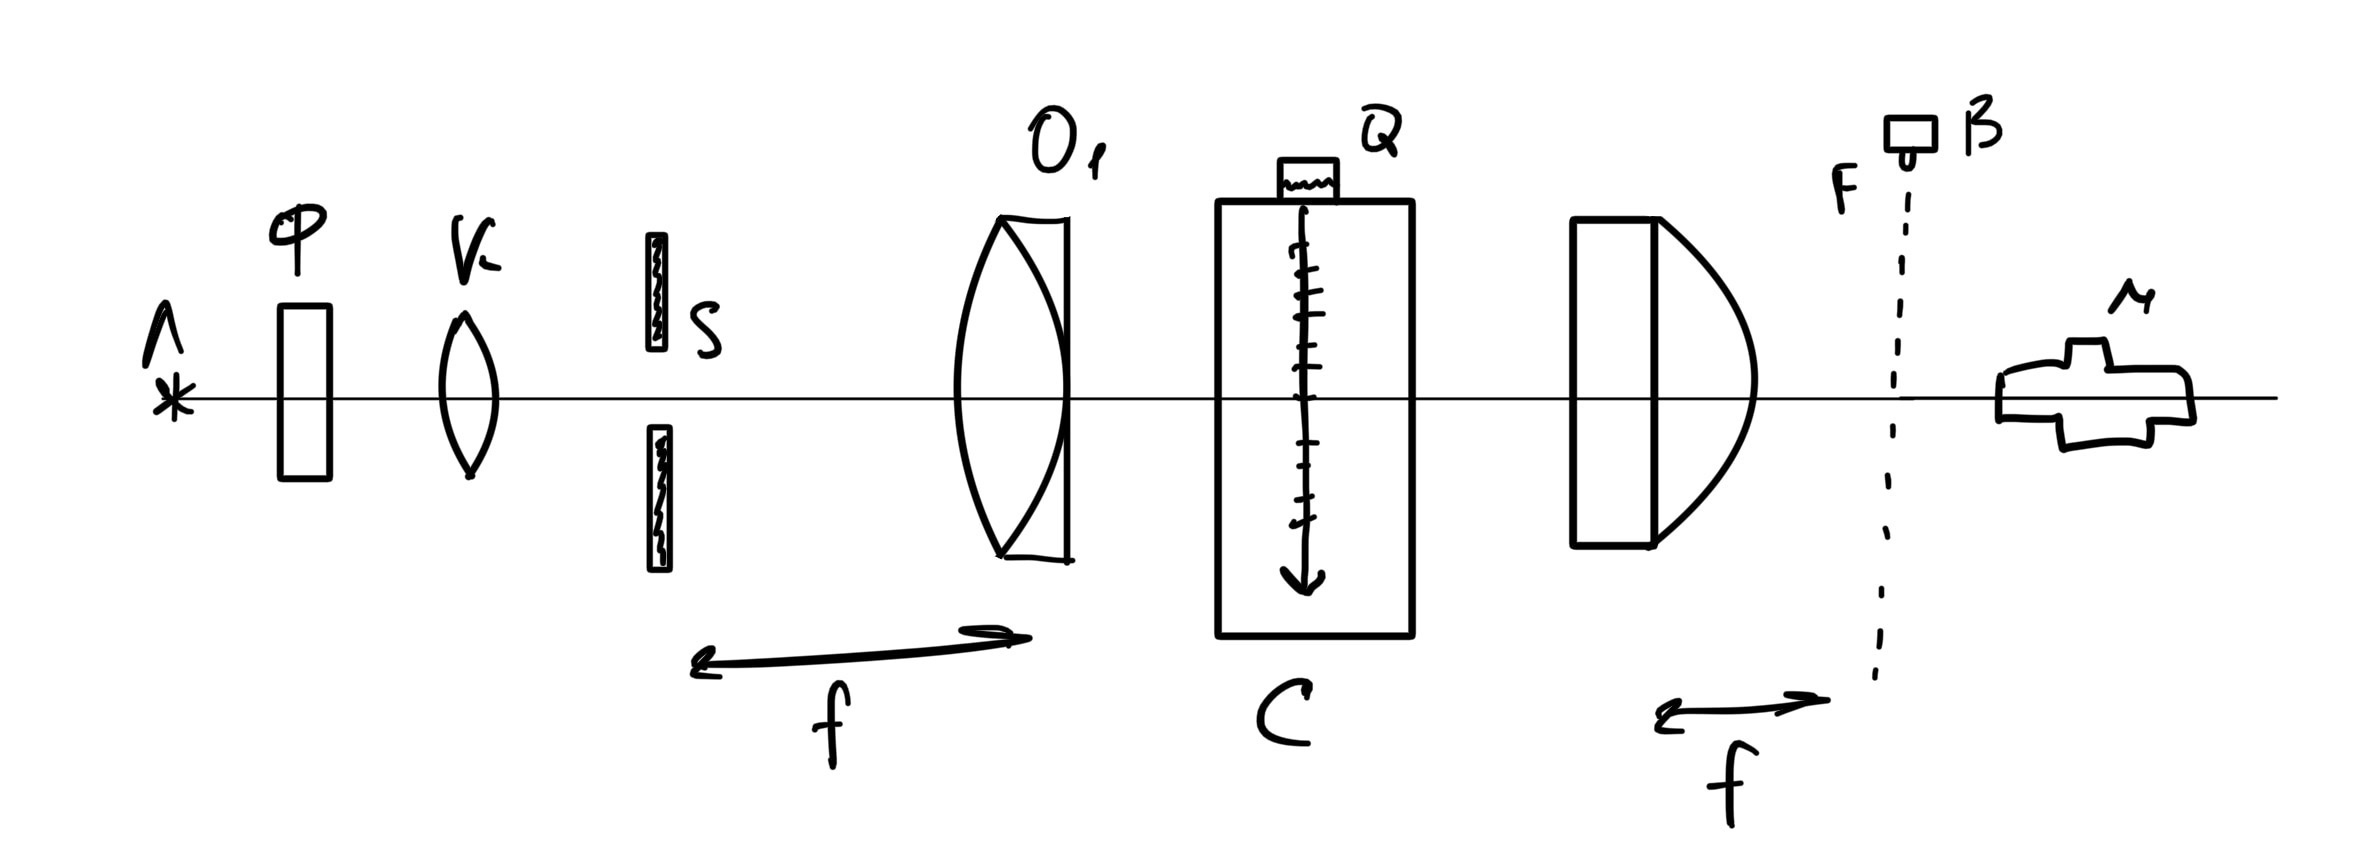
\includegraphics[width=1\textwidth]{set}
    \caption{Схема установки}
    \label{fig:set}
\end{figure}

Источник света Л через светофильтр Ф и конденсор К освещает щель $S$, которая расположена в фокусе объектива $\mathrm{O}_1$. Выходящий из объектива параллельный пучок света проходит через кювету $C$ перпендикулярно направлению распространения УЗ-волн. Эти волны возбуждаются в жидкости пьезокварцевой пластинкой $Q$, прикреплённой к стенке кюветы. На кварцевую пластинку подаётся синусоидальное напряжение ультразвуковой частоты от генератора (на рис. не показан). В результате взаимодействия света с ультразвуковой волной в фокальной плоскости второго объектива $\mathrm{O}_2$ образуется дифракционная картина, наблюдаемая при помощи микроскопа М. При этом обязательно применяют монохроматическое излучение (красный светофильтр).

Дифракционные полосы ориентированы горизонтально. Расстояние между ними можно измерить с помощью специального отсчётного устройства с микрометрическим винтом В. Этот винт передвигает размещённые на стекле отсчётного устройства тонкую реперную линию Рл, перекрестие $\Pi$ и толстую проволоку Пр, которая используется в методе тёмного поля. Все измерительные линии должны быть расположены в плоскости $F$ резкого изображения щели.

Чёткость дифракционньх полос зависит от ряда факторов, например, от ширины щели $S$, от её наклона по отношению к вертикали, от угла наклона кюветы к падающему лучу и т. д.
Длина $\Lambda$ ультразвуковой волны определяется по формуле
\begin{equation}
\Lambda \sin \Theta_m=m \lambda
\end{equation}
в силу малости углов $\Theta_m$ окончательное выражение может быть представлено в виде
\begin{equation}
l_m=m f \frac{\lambda}{\Lambda}
\end{equation}
где $l_m-$ измеренное на опыте линейное расстояние между $m$-м и нулевым максимумами, а $f$ - фокусное расстояние объектива $\mathrm{O}_2$.

Скорость $\nu$ распространения звука в воде можно рассчитать, если известна частота $\nu$ кварцевого излучателя:
\begin{equation}
v=\Lambda \nu
\end{equation}

\section{Ход работы}
\subsection*{Определение скорости ультразвука по дифракционной картине}

Оценим \emph{по порядку величины} скорость звука как удвоенное расстояние между наиболее чёткими дифракционными картинами:
\begin{equation*}
	n = 66, \Lambda \approx 1316 \text{ мкм}
\end{equation*}
Рабочая частота 1,3 МГц, тогда скорость
\begin{equation*}
	v \approx \Lambda \nu = 1718 \text{ м/c}
\end{equation*}
Определим положения дифракционных полос. Для этого для нескольких частот зафиксируем дифракционные картины на фото и определим $l_m$.
Далее по формуле (2) найдем $\Lambda$, учитывая $\lambda = 640 $ нм, $f = 28 $ см: 

\begin{equation}
	\Lambda = \frac{m f \lambda}{l_m}
\end{equation}

\begin{table}[H]
	\centering
	\begin{tabular}{|c|c|c|c|}
	\hline
	\textbf{m} & \textbf{$\Lambda, \text{ мкм}$} & \textbf{$\nu, \text{МГц}$} & \textbf{$v, \text{ м/с}$} \\ \hline
	3          & 1358                            & 1,0                        & 1417                      \\ \hline
	3          & 1211                            & 1,2                        & 1452                      \\ \hline
	3          & 1088                            & 1,3                        & 1442                      \\ \hline
	3          & 946                             & 1,5                        & 1404                      \\ \hline
	\end{tabular}
	\caption{Скорости звука}
	\label{tab:my-table}
\end{table}
Тогда среднее 
\begin{equation*}
	v = 1429 \pm 50 \text{ м/с}
\end{equation*}

\subsection*{Определение скорости ультразвука методом тёмного поля}

Проведем калибровку: поставим пластинку с калибровочной сеткой. Длина стороны 1 мм соотвествует 21 делению, значит цена деления шкалы микроскопа 1/21 мм.

Закроем проволокой центральный максимум и определим период полученной решетки при фиксированных частотах. Зафиксируем с помощью окулярной шкалы микроскопа разность координат N первой и последней из хорошо видимых в поле зрения тёмных полос
и количество m светлых промежутков между ними. По полученным данным рассчитаем длину волны $\Lambda$, построим график зависимости $\Lambda = f(1/\nu)$ и по коэффициенту наклона прямой определим скорость звука в воде.
	
\begin{table}[H]
	\centering
	\begin{tabular}{|c|c|c|c|}
	\hline
	\textbf{$\nu,   \text{ МГц}$} & \textbf{$N, \text{ мм}$} & \textbf{m} & \textbf{$\Lambda, \text{ мкм}$} \\ \hline
	1,1                           & 7,476                    & 11         & 1495                           \\ \hline
	1,2                           & 7,619                    & 12         & 1385                           \\ \hline
	1,3                           & 7,048                    & 12         & 1175                           \\ \hline
	1,4                           & 5,952                    & 11         & 1190                           \\ \hline
	1,5                           & 5,571                    & 11         & 1114                           \\ \hline
	1,6                           & 5,667                    & 12         & 1030                           \\ \hline
	\end{tabular}
	\caption{Данные с метода темного поля}
	\label{tab:m}
\end{table}

\begin{figure}[H]
    \centering
    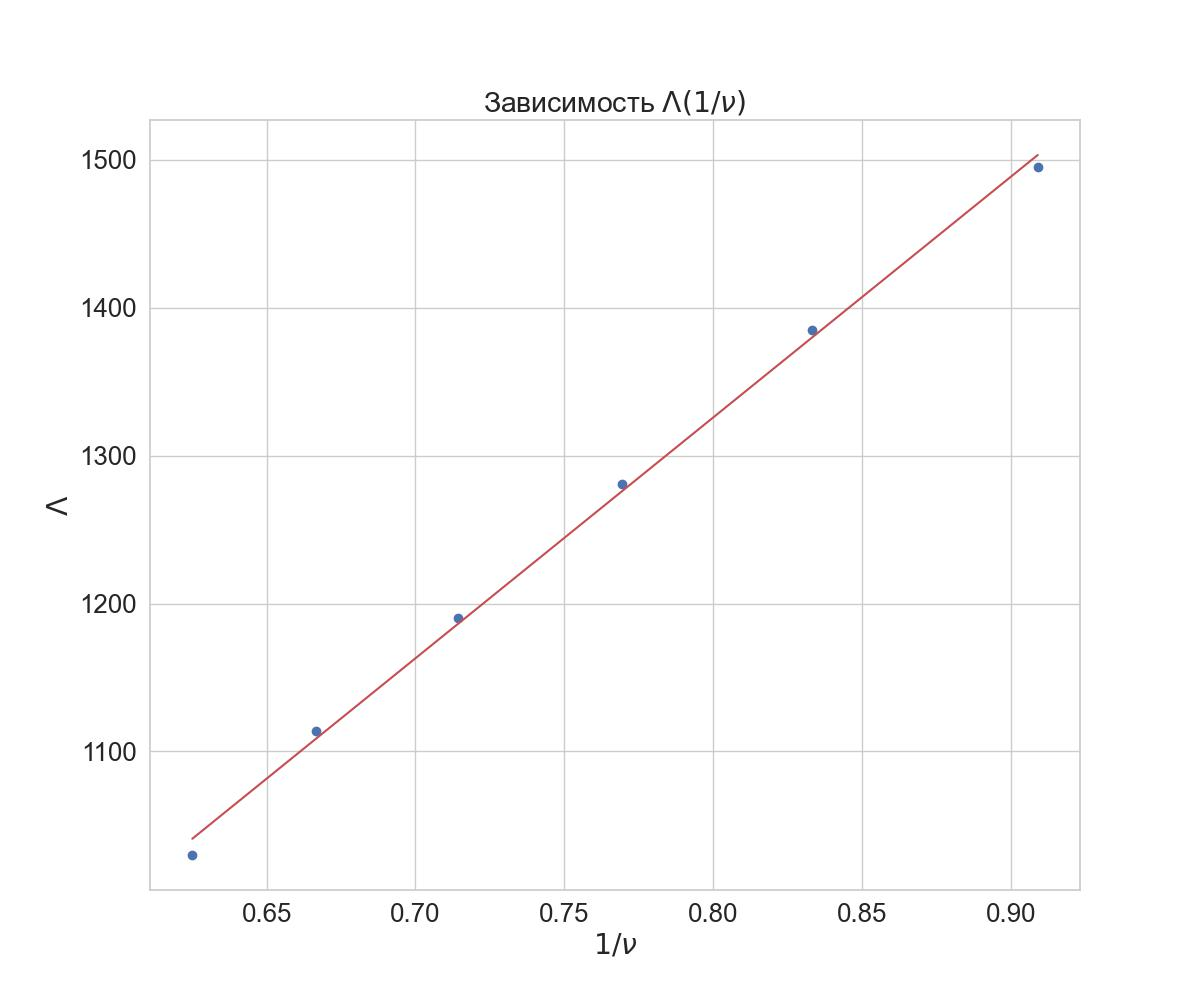
\includegraphics[width=1\textwidth]{plot1.jpg}
    \caption{График по методу темного поля}
    \label{fig:plot1}
\end{figure}
Итого:
\begin{equation*}
	v = 1627 \pm 40 \text{ м/с}
\end{equation*}

\section{Выводы}
Если считать, что скорость звука в воде равна 1500 м/c, то ближе к истине оказался первый метод. Но в целом, оба значения получились неплохие.
\begin{table}[H]
	\centering
	\begin{tabular}{|c|c|}
	\hline
	\textbf{Метод}        & \textbf{$v, \text{ м/c}$} \\ \hline
	Дифракционная картина & $1429 \pm 50$             \\ \hline
	Тёмное поле           & $1627 \pm 40$             \\ \hline
	\end{tabular}
	\caption{Итоги}
	\label{itog}
	\end{table}
\end{document}